\documentclass{beamer}


\mode<presentation>
{
  \usetheme{CambridgeUS}
	\usecolortheme{beaver}
  % or ...

  \setbeamercovered{transparent}
  % or whatever (possibly just delete it)
}


\usepackage{xeCJK}
\usepackage[english]{babel}
\usepackage[utf8]{inputenc}
\usepackage{times}
\usepackage[T1]{fontenc}
\usepackage{hyperref}
\usepackage{pifont}
\usepackage{bibentry}
\usepackage{verbatim}
\usepackage{fontspec}
\newcommand{\cmark}{\ding{51}}%
\newcommand{\xmark}{\ding{55}}%
\setCJKmainfont{WenQuanYi Micro Hei}
\setmainfont{DejaVu Sans}


\title[开源软件基础] 
{开源软件基础}
\subtitle{Git与版本控制}

\author[Zhilei Ren] 
{Zhilei Ren}

\institute[OSCAR Team] % (optional, but mostly needed)
{
\\
\includegraphics[width=0.2\textwidth]{../../utils/logo.jpg}\\
OSCAR Team, School of Software, 
Dalian University of Technology
}


\subject{Open source software}

\pgfdeclareimage[height=0.5cm]{university-logo}{../../utils/logo.jpg}
\logo{\pgfuseimage{university-logo}}



% Delete this, if you do not want the table of contents to pop up at
% the beginning of each subsection:
\AtBeginSubsection[]
{
  \begin{frame}<beamer>{Outline}
    \tableofcontents[currentsection,currentsubsection]
  \end{frame}
}


% If you wish to uncover everything in a step-wise fashion, uncomment
% the following command: 

%\beamerdefaultoverlayspecification{<+->}

\setbeamertemplate{section in toc}[circle]
\setbeamertemplate{items}[circle]
\setbeamertemplate{caption}[numbered]
\setbeamertemplate{bibliography item}{\insertbiblabel}
\setbeamertemplate{bibliography entry title}{}
\setbeamertemplate{bibliography entry journal}{}

\begin{document}

\begin{frame}
  \titlepage
\end{frame}

%\begin{frame}{Outline}
%  \tableofcontents[currentsection,currentsubsection, 
%    hideothersubsections, 
%    sectionstyle=show,
%]
%\end{frame}

\AtBeginSection[]
{
 \begin{frame}<beamer>
 \frametitle{Outline}
 \tableofcontents[currentsection]
 \end{frame}
}
\section{Before Git}
\begin{frame}[t]{Vim}
	\begin{block}{Why Vim}
\begin{itemize}
	\item 用于提交commit信息（非必要）
	\item 用于解决冲突（非必要）
	\item 那为什么？
\end{itemize}
	\end{block}
\end{frame}
\begin{frame}[t]{编辑器效率对比}
	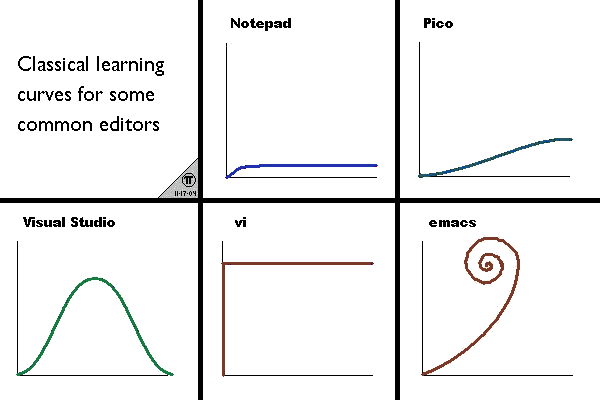
\includegraphics[width=.5\textwidth]{vim-learning.jpg}
\end{frame}
\begin{frame}[t]{编辑器效率对比}
	
\includegraphics[width=.5\textwidth]{curve.png}
\end{frame}
\begin{frame}
  \frametitle{Real Programmer\footnote{\url{https://www.xkcd.com/378/}}}
	\centering
	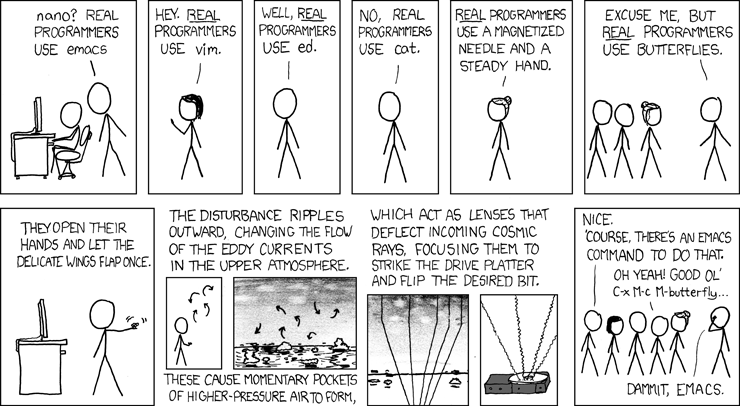
\includegraphics[width=.7\textwidth]{real-programmers.png}
\end{frame}
\begin{frame}
	\frametitle{今天就能开始用的小知识}
	\begin{block}
		{开源软件中的Diss与Respect}
		\begin{itemize}
			\item vi by Bill Joy
			\item vim by Bram Moolenaar
			\item neovim by Thiago de Arruda\footnote{\url{https://geoff.greer.fm/2015/01/15/why-neovim-is-better-than-vim/}}
		\end{itemize}
	\end{block}
	
\end{frame}
\begin{frame}
  \frametitle{Bram Moolenaar on neovim}
	\begin{block}
		{}
		It's going to be an awful lot of work, with the result that not all 
		systems will be supported, new bugs introduced and what's the gain 
		for the end user exactly? 

		Total refactoring is not a solution.  It's much better to improve what 
		we have.  Perhaps with some small refactorings specifically aimed at 
		making Vim work better for users.\footnote{\url{https://groups.google.com/forum/m/\#!topic/vim\_dev/x0BF9Y0Uby8}}
\end{block}
	
\end{frame}
\begin{frame}[t]{高效编辑}
	\begin{itemize}
		\item 基于模式
		\item 高效移动
		\item 命令组合
		\item 自定义/绑定
	\end{itemize}
\end{frame}
\begin{frame}[t]{Vim模式}
	\centering
	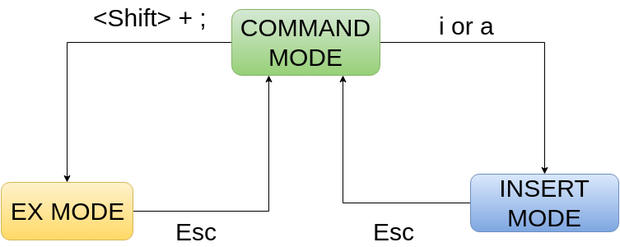
\includegraphics[width=.5\textwidth]{vimmodes.png}
\end{frame}
\begin{frame}[t]{高效移动}
	\centering
	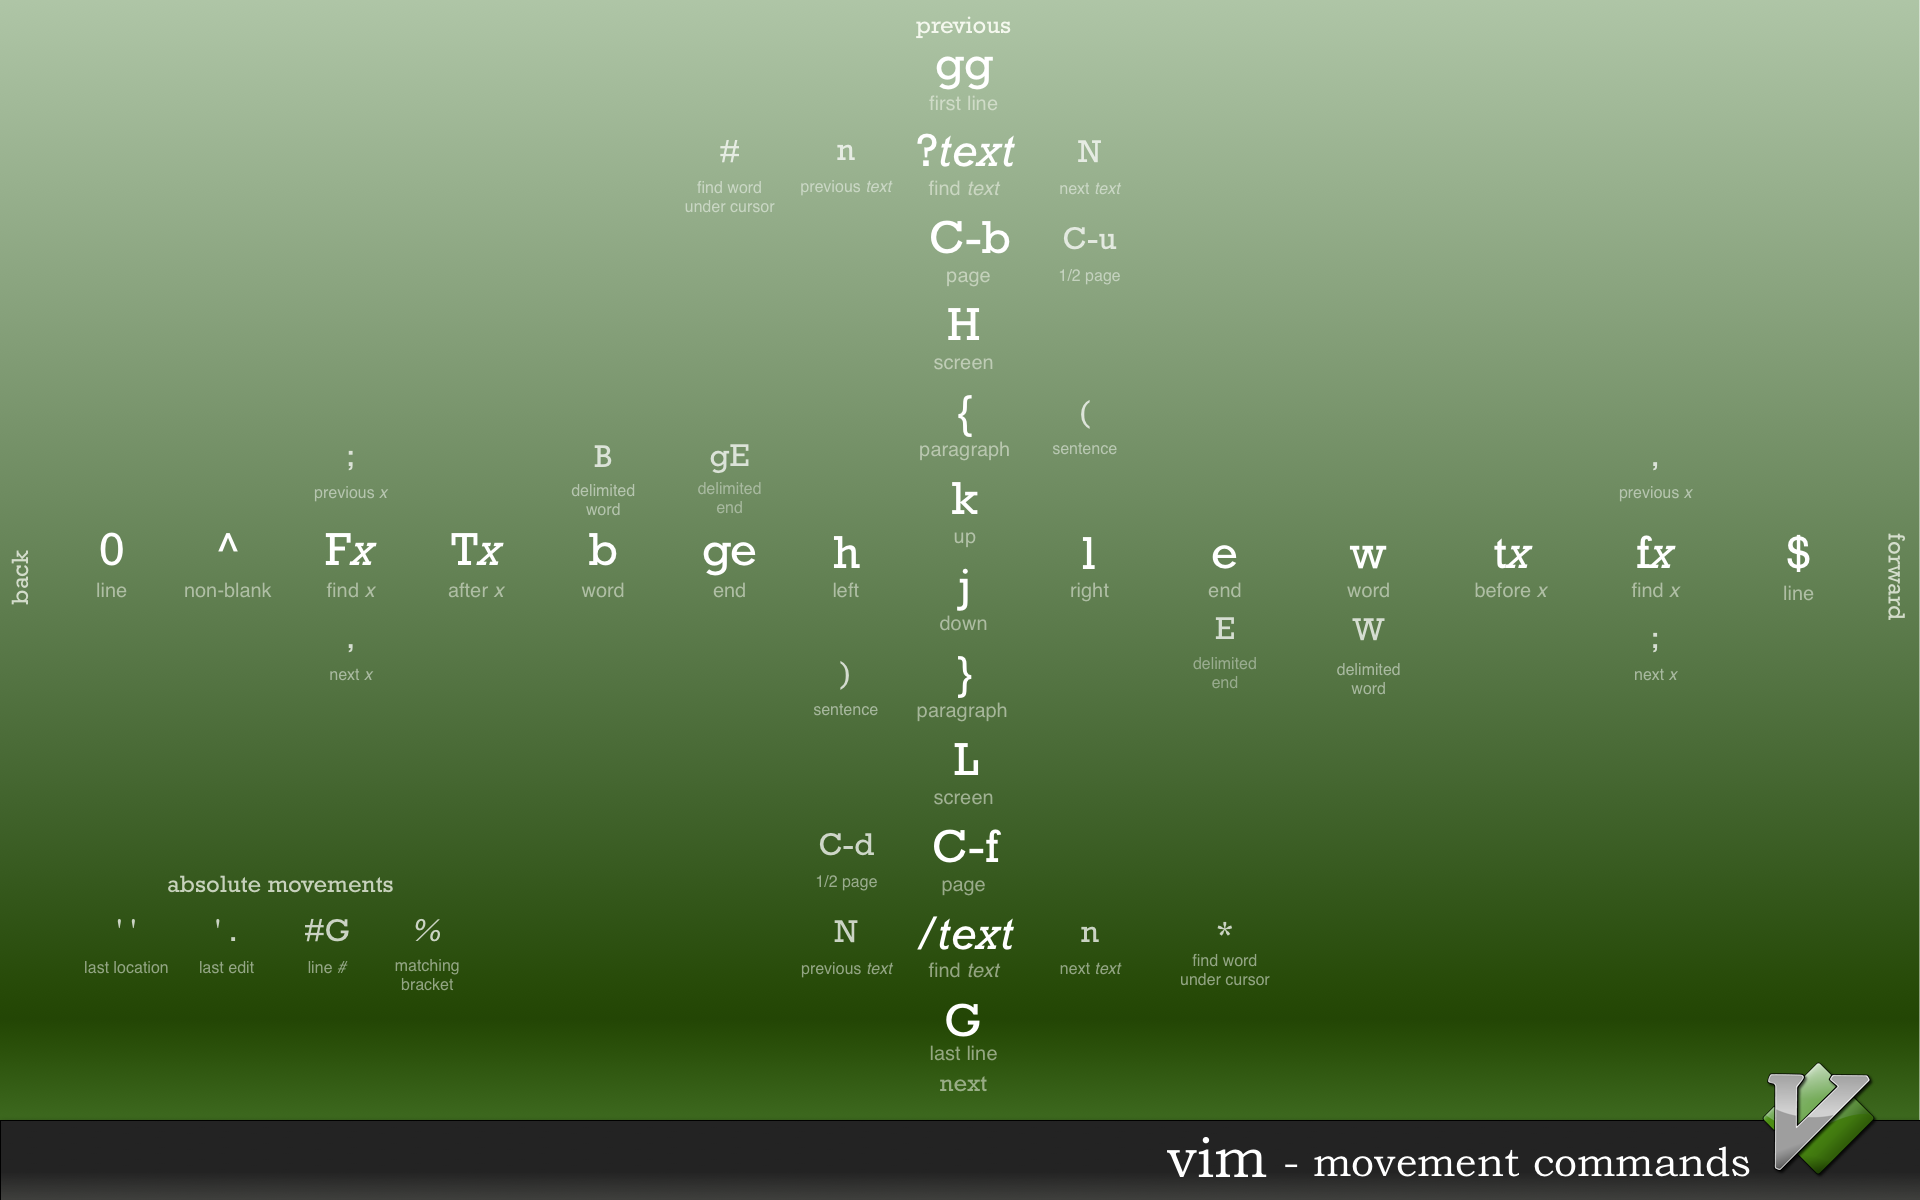
\includegraphics[width=.8\textwidth]{movement.png}
\end{frame}
\begin{frame}[t]{高效移动}
    \centering
    \Huge
    \scalebox{2}{
    \color{blue}H \color{red}J \color{blue}K \color{red}L
    }

    \scalebox{2}{
    \color{blue}$\leftarrow$ \color{red}$\downarrow$ \color{blue}$\uparrow$ \color{red}$\rightarrow$
    }
\end{frame}
\begin{frame}[t]{高效编辑}
    \centering
    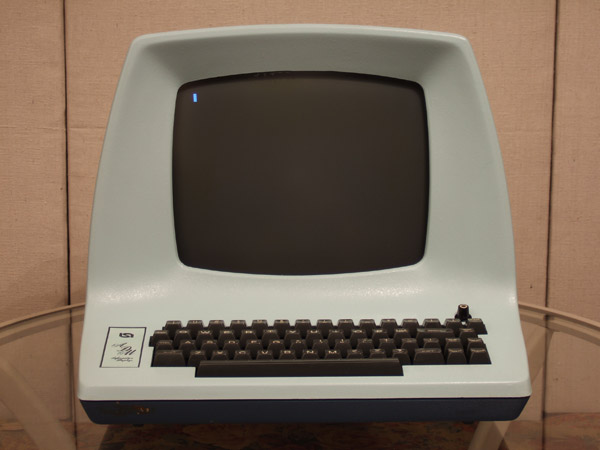
\includegraphics[width=.5\textwidth]{lsiadm3a.jpg}
    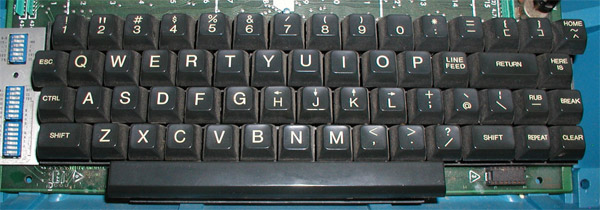
\includegraphics[width=.5\textwidth]{keyboard.jpg}
    
\end{frame}
\begin{frame}[t]{移动}
        \begin{itemize}
            \item gg: goto first line
            \item G: goto last line
            \item 0: goto first column
            \item \^{}: goto first non-blank column
            \item \$: goto last column 
            \item w: next word
            \item W: next Word
            \item e: end of word
            \item E: end of Word
            \item fa: find a in current line
            \item Fa: find a in current line backward
            \item ta: find till before a 
            \item Ta: find till before a backward
        \end{itemize}
\end{frame}
\begin{frame}[t]{单独使用命令}
    \begin{block}
        {}
        \begin{itemize}
            \item i: insert
            \item I: insert at front
            \item a: append
            \item A: append after end
            \item o: append new line
            \item O: insert new line
        \end{itemize}
    \end{block}
\end{frame}
\begin{frame}[t]{命令与文本对象}
	\begin{block}{命令}
		\begin{itemize}
			\item c: Change
			\item d: Delete
			\item y: Yank
			\item gU: Upper case
			\item gu: Lower case
			\item g$\sim$: Switch case
			\ldots
		\end{itemize}
	\end{block}
	\begin{block}{文本对象}
		\begin{itemize}
			\item aw: a word
			\item iw: inner word
			\item ab: a bracket
			\item ib: inner bracket
			\item at: a tag
			\item it: inner tag
			\ldots
		\end{itemize}
	\end{block}
\end{frame}
\begin{frame}[t]{合体（误）}
	\Huge
	\color{red}{命令}+\color{blue}{移动}/\color{green}{文本对象}
	\large
	\vspace{2cm}
	\begin{itemize}
		\item \color{red}{d}\color{blue}{j}\color{black}: delete current and the next lines
		\item \color{red}{y}\color{blue}\color{blue}0\color{black}: copy to the line head
		\item \color{red}{c}\color{green}iw\color{black}: change inner word
		\item \color{red}{d}\color{green}ab\color{black}: delete a bracket
		\item \color{red}{gU}\color{green}it\color{black}: change inner tag to lower case
		\ldots
	\end{itemize}
\end{frame}
\begin{frame}[t]{今天就能开始用的小知识}
    \begin{block}{表妹}
        {\scriptsize CNLabelContactRelationYoungerCousinMothersSiblingsDaughterOrFathersSistersDaughter}\footnote{\tiny \url{https://developer.apple.com/documentation/contacts/cnlabelcontactrelationyoungercousinmotherssiblingsdaughterorfatherssistersdaughter}}\footnote{\tiny{\url{https://news.ycombinator.com/item?id=20341855}}}

        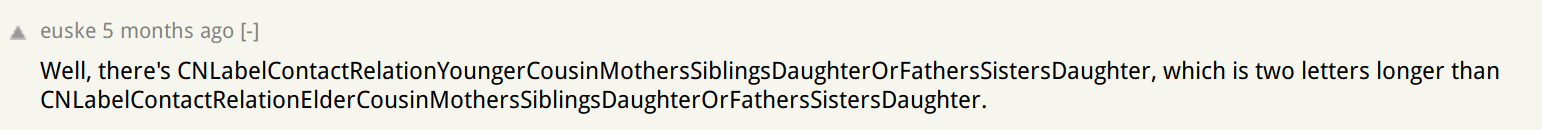
\includegraphics[width=.8\textwidth]{elder.png}
        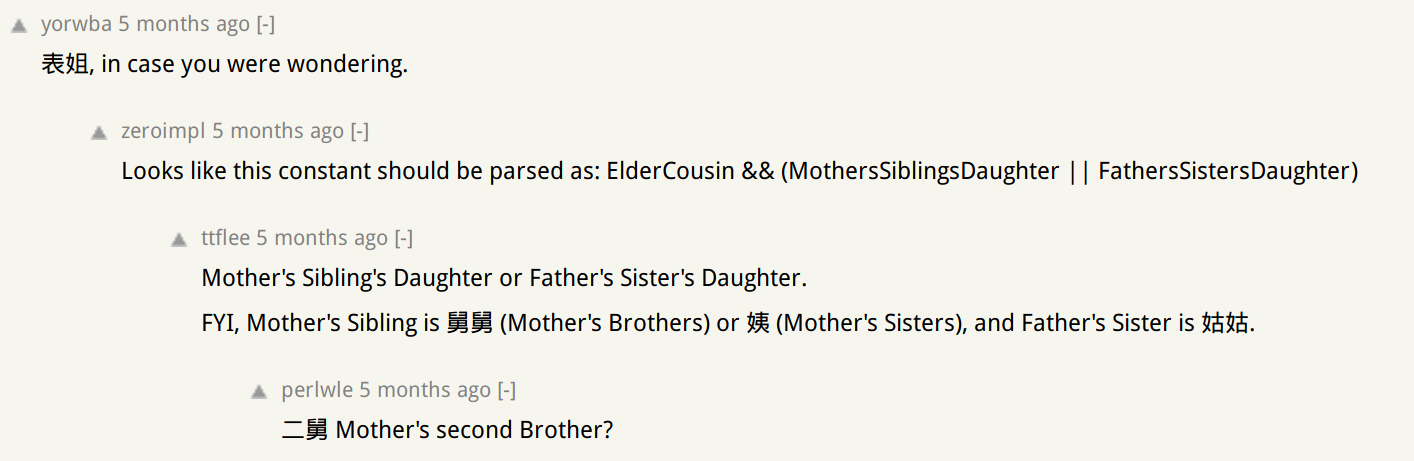
\includegraphics[width=.8\textwidth]{hn.png}
    \end{block}
    

    
    
\end{frame}
\begin{frame}[t]{命令行模式}
    \begin{block}
        {相对高阶功能}
        \begin{itemize}
            \item :\%s/re.pattern/replace/g 全局替换
            \item :g/re.pattern/d 删除匹配行
            \item :h! E478 Don't panic
            \item :h 42

What is the meaning of life, the universe and everything?  *42*

Douglas Adams, the only person who knew what this question really was about is
now dead, unfortunately.  So now you might wonder what the meaning of death
is...
        \end{itemize}
    \end{block}
\end{frame}
\begin{frame}[t]{书籍推荐（伪）}
    
\includegraphics[height=.5\textwidth]{hhgg-ultimate-soft.jpg}
    
\includegraphics[height=.5\textwidth]{Marvin.jpg}
\end{frame}
\begin{frame}[t]{Practise makes perfect}
	\normalsize
	\begin{block}{继续学习}
\begin{itemize}
	\item vimtutor
	\item vimcasts\footnote{\url{http://vimcasts.org/}}
	\item 7 Habits For Effective Text Editing\footnote{\url{http://v.youku.com/v_show/id_XMTIwNDY5MjY4.html?spm=a2h0k.8191407.0.0&from=s1.8-1-1.2}}
	\item Maybe emacs\footnote{\url{https://www.bilibili.com/video/av6048518/?from=search&seid=12030402565005031700}}
\end{itemize}
	\end{block}
	
\end{frame}
\section{Git入门} % (fold)
\label{sec:Git入门}
\begin{frame}[t]{Why Git\footnote{\url{http://phdcomics.com/comics/archive.php?comicid=1323}}}
    \centering
    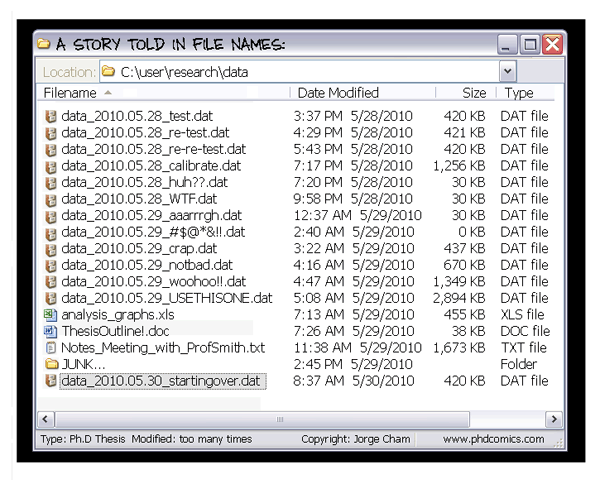
\includegraphics[width=.7\textwidth]{filename.png}
\end{frame}
\begin{frame}[t]{Why Git\footnote{\url{http://phdcomics.com/comics/archive.php?comicid=1531}}}
    \centering
    
\includegraphics[width=.4\textwidth]{final.png}
\end{frame}
\begin{frame}[t]{Git}
    \begin{block}
        {}
git是一个分布式版本控制软件，最初由林纳斯·托瓦兹创作，于2005年以GPL发布。最初目的是为更好地管理Linux内核开发而设计。

git最初的开发动力来自于BitKeeper和Monotone。很多著名的软件都使用git进行版本控制，其中包括Linux内核、X.Org服务器和OLPC内核等项目的开发流程。
    \end{block}
\end{frame}
\begin{frame}[t]{今天就能开始用的小知识}
    \begin{block}
        {Git名字的由来}
        林纳斯·托瓦兹自嘲地取了这个名字“git”，该词源自英国俚语，意思大约是“混账”。\footnote{\url{https://git.wiki.kernel.org/index.php/GitFaq}}

I'm an egotistical bastard, and I name all my projects after myself. First Linux, now git.	
    \end{block}
\end{frame}
\begin{frame}[t]{Git命令初步}
	\centering
    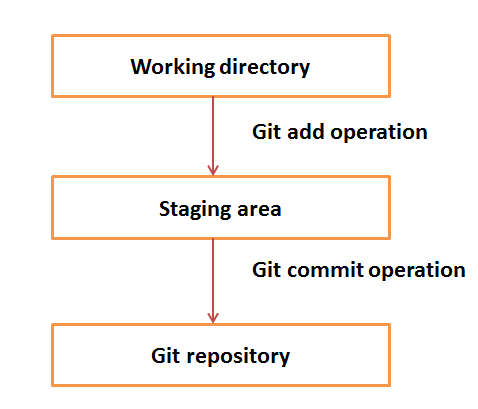
\includegraphics[width=.5\textwidth]{staging-area.png}
    
\end{frame}
\begin{frame}[t,fragile]{Git命令初步}
    \scriptsize
\begin{verbatim}
#initialization
$ git init

#configuration
$ git config --global user.name "Your Name"
$ git config --global user.email "you@your.server"

# First commit
$ git add example.py

# adds file to the staging area
$ git commit -m "First commit"

# Second commit
$ git add another.py

# adds file to the staging area
$ git commit -m "Second commit"        
\end{verbatim}
    
\end{frame}

\begin{frame}{Branching and Merging}
\begin{itemize}
   \item By default you are on the "master" branch
   \item To create a new branch and switch to it:
  \begin{itemize}
    \item \$ git branch branchName
    \item \$ git checkout branchName
  \end{itemize}
   \item Merge changes back to master branch
  \begin{itemize}
     \item \$ git checkout master
     \item \$ git merge branchName
     \item To delete branch
    \begin{itemize}
      \item \$ git branch -d branchName
    \end{itemize}
  \end{itemize}
\end{itemize}
\end{frame}

\begin{frame}{My Typical Git Workflow}
  \begin{itemize}
     \item Master branch is always clean and working
     \item When I want to try a new idea, create a branch
     \item Work and commit to that branch until code is clean and working
     \item Switch back to master and merge branch into master
     \item Delete branch
  \end{itemize}
\end{frame}

\begin{frame}{Things to Keep in Mind}
  \begin{itemize}
     \item Any branch can be merged to any other branch
    \begin{itemize}
      \item Careful, this might get confusing
    \end{itemize}
     \item Must commit before switching branches
     \item Unless you add it, a file will not be tracked.
     \item If you want to ignore a file, add it to the
    .git/info/exclude file.
     \item To revert a file back to it's state at the last commit:
    \begin{itemize}
      \item git checkout fileName
    \end{itemize}
     \item To revert the entire repo to it's state at the last commit:
    \begin{itemize}
      \item git reset --hard HEAD
      \item CAREFULL! You'll loose all your changes since your last commit!
    \end{itemize}
   \item \url{http://git-scm.com/}
  \end{itemize}
\end{frame}

\begin{frame}{Things to Keep in Mind}
  \begin{itemize}
      \item git存储整个文件，而非diff
      \item 网络搜索并不可靠
  \end{itemize}

  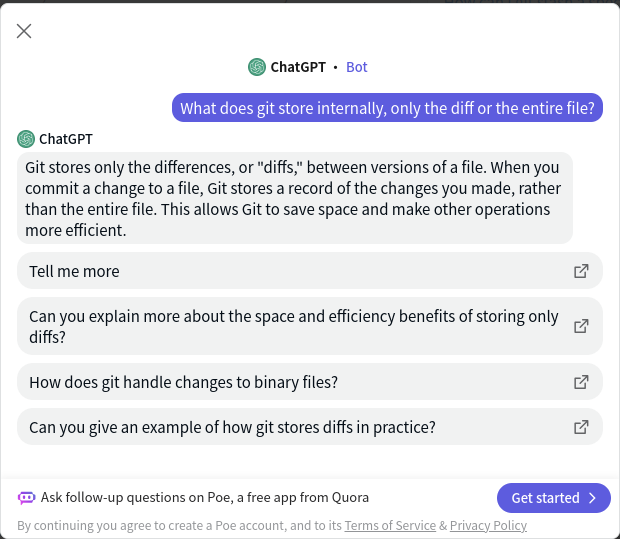
\includegraphics[width=.5\textwidth]{git-chat.png}
\end{frame}

% section Git入门 (end)



\end{document}
